\documentclass[12pt,a4paper]{article}
\usepackage[utf8]{inputenc}
\usepackage[russian,english]{babel}

\usepackage{amsmath}
\usepackage{amsfonts}
\usepackage{amssymb}
\usepackage{array}
\usepackage{graphicx} % Required to insert images
\usepackage{float}
\usepackage[left=2cm,right=2cm,top=2cm,bottom=2cm]{geometry}


\usepackage{biblatex}

\usepackage[normalem]{ulem} %for underline
\usepackage[usenames,dvipsnames]{color} % Required for custom colors
\definecolor{MyBlue}{rgb}{0.0,0.3,0.7} 
\definecolor{MyRed}{rgb}{0.75, 0.12, 0.20} 
\definecolor{UURed}{rgb}{0.75, 0.12, 0.20} 
\newcommand{\definition}[1]{ \textcolor{MyRed}{\uline{\textbf {#1}}}}% For writing
\newcommand{\example}[1]{\textcolor{MyBlue}{\textbf{Example {#1}: }}}

%----------------------------------------------------------------------------------------
%	TITLE PAGE
%----------------------------------------------------------------------------------------

\newcommand*{\titleAT}{\begingroup % Create the command for including the title page in the document
\newlength{\drop} % Command for generating a specific amount of whitespace
\drop=0.1\textheight % Define the command as 10% of the total text height

\rule{\textwidth}{1pt}\par % Thick horizontal line
\vspace{2pt}\vspace{-\baselineskip} % Whitespace between lines
\rule{\textwidth}{0.4pt}\par % Thin horizontal line

\vspace{\drop} % Whitespace between the top lines and title
\centering % Center all text
\textcolor{UURed}{ % Red font color
{\Huge \textbf{Data Reduction}}\\[0.75\baselineskip] % Title line 1
{\Huge \textit{\&}}\\[0.75\baselineskip] % Title line 2
{\Huge \textbf{Error Analysis}}\\[0.75\baselineskip]
{\Large \textit{in brief}}} % Title line 3


\vspace{0.10\drop} % Whitespace between the title and short horizontal line
\rule{0.3\textwidth}{0.4pt}\par % Short horizontal line under the title
\vspace{\drop} % Whitespace between the thin horizontal line and the author name

{\Large \textsc Anna Sinelnikova}\par % Author name

\vfill % Whitespace between the author name and publisher text
%{\large \textcolor{Red}{\plogo}}\\[0.5\baselineskip] % Publisher logo
\begin{figure}[H]
\centering

\includegraphics[width=0.3\linewidth]{Uppsala_University_seal.pdf}
\end{figure}
{\large \textsc{Uppsala University\\2017}}\par % Publisher

\vspace*{\drop} % Whitespace under the publisher text

\rule{\textwidth}{0.4pt}\par % Thin horizontal line
\vspace{2pt}\vspace{-\baselineskip} % Whitespace between lines
\rule{\textwidth}{1pt}\par % Thick horizontal line

\endgroup}

%----------------------------------------------------------------------------------------
%																											BEGIN
%----------------------------------------------------------------------------------------
\begin{document}
\thispagestyle{empty} % Removes page numbers
\titleAT

\newpage
\tableofcontents
\newpage

%----------------------------------------------------------------------------------------
%	Introduction
%----------------------------------------------------------------------------------------
\section*{Introduction}
This booklet was written to give an idea about how errors propagate in physical measurements.
For this purpose we will first discuss what a measurement of a physical quantity means and where errors come from. Then we will show how to write down the result in a proper way, using a scientific notation. We then discuss how to compute errors in different cases, in direct and indirect measurements. Finally, we give an example that explicitly shows how to use the methods.

The booklet can be useful for students who do laboratory work in physics. It might be used as a reference source for data reduction and propagation of errors.

%----------------------------------------------------------------------------------------
%	Why Do We Calculate Errors?
%----------------------------------------------------------------------------------------
\section{Why Do We Calculate Errors?}
When we solve problems, our aim can be to find some number. This number is the answer to a question like: ``how many?", ``how long?", ``how much time?" etc. In physical problems the question can be: ``what force?"
, ``what mass?" ... In all these examples we want to find \textit{one exact number}. This number is the solution for the problem.

When we do an experiment we might also be interested in numbers that answer the same questions as above, but now instead of using a mathematical model we have to deal with real world. What is the difference?

We cannot measure anything with infinite precision in reality. This restriction is unavoidable. We can improve our devices and it can give us better and better precision, but we cannot reach this limit. So whatever we measure, we need to state
how trustful the result is, i.e. how close it to the ``true" value.

The quality of an experiment is defined by the value of the error. It is quite clear that if the uncertainty is larger than the found value itself, then the result of such experiment does not make any sense at all.

For example, one of the biggest discoveries of our century in physics was the first direct observation of gravitational waves by LIGO (Laser Interferometer Gravitational-Wave Observatory) on September 14, 2015\footnote{Nature News. doi:10.1038/nature.2016.19361. Retrieved 11 February 2016}. The experiments at LIGO started in 2002, more than 10 years ago. The theoretical predictions were made one century ago. The issue was the precision of the experiment. The errors (which were produced by noise) were larger than the expected value. It took one hundred years to invent and conduct the experiment where the result could be trusted, i.e. with small enough errors.

Error propagation in not an independent science. It uses different branches of statistics, depending on what experiment you have. That fact probably makes things even more complicated.

%----------------------------------------------------------------------------------------
%	Physical Quantity and its Measurement
%----------------------------------------------------------------------------------------
\section{Physical Quantity and its Measurement}

\definition{A physical quantity} is a quantitative property of a phenomenon, body, or substance.
Each physical quantity must be defined such that it unequivocally can be found experimentally, or theoretically, in any real situation. The value of a physical quantity can be expressed as a combination of a magnitude expressed by a number and a unit.
 \newline
\newline
\definition{Measurement of a physical quantity} is the determination or estimation of how many uniform physical quantities are contained in it. Physical quantities are uniform if they describe the same properties and differ only by value. Usually as uniform physical quantities we take a measurement unit. Units of measurement are defined and adopted by convention or by law and form a system of units.

\example{} Kilometre, metre, millimetre are units of length. Hence they are uniform. When you want to find the length of any object you have to find how many units of length are contained in the object. In the International System of Units (SI) the definition of a metre is: Length of the path travelled by light in a vacuum in 1/299 792 458 of a second.
\newline
\newline
\definition{Measurement error} (or Observational error) is the difference between a measured value of a quantity and its true value. The problem is that we do not know the true value, if we did there would be no reason to perform the experiment. Hence we need a way to systematically estimate errors both from data and from experimental conditions.


\textbf{Errors have the same measurement units as the value itself!}

%----------------------------------------------------------------------------------------
%	Errors Classifications
%----------------------------------------------------------------------------------------
\section{Classification of errors}
There are different ways of classifying errors. We will consider two of them here.

\subsection{Classification of errors by nature of their occurrence}
\definition{Random errors} are errors which are caused by uncontrolled fluctuations in observations which appear randomly in each measurement. This type of errors can be estimated by repeating the same experiment several times and using statistical analysis. We can decrease this error by increasing the number of measurements. In this case we say that we increase the \definition{precision} of the measurement value. Random errors vanish when the number of measurements is taken to infinity.
\newline
\newline
\definition{Systematic errors} are constant or change according to some law during the experiment. The reason for this type of errors is errors in the tools we use in the experiment, both equipment and methods of measurement. This kind of errors can be decreased only by improving the tools themselves. We then say that we increase the \definition{accuracy} of the measurement value (see fig. \ref{fig:accuracy} for comparison accuracy and precision). There is no way to avoid systematic errors in any real experiment.  The best way to reveal these errors is to measure the same quantity with completely different methods in completely different experiments.

\begin{figure}
	\centering
	\vskip -2cm
	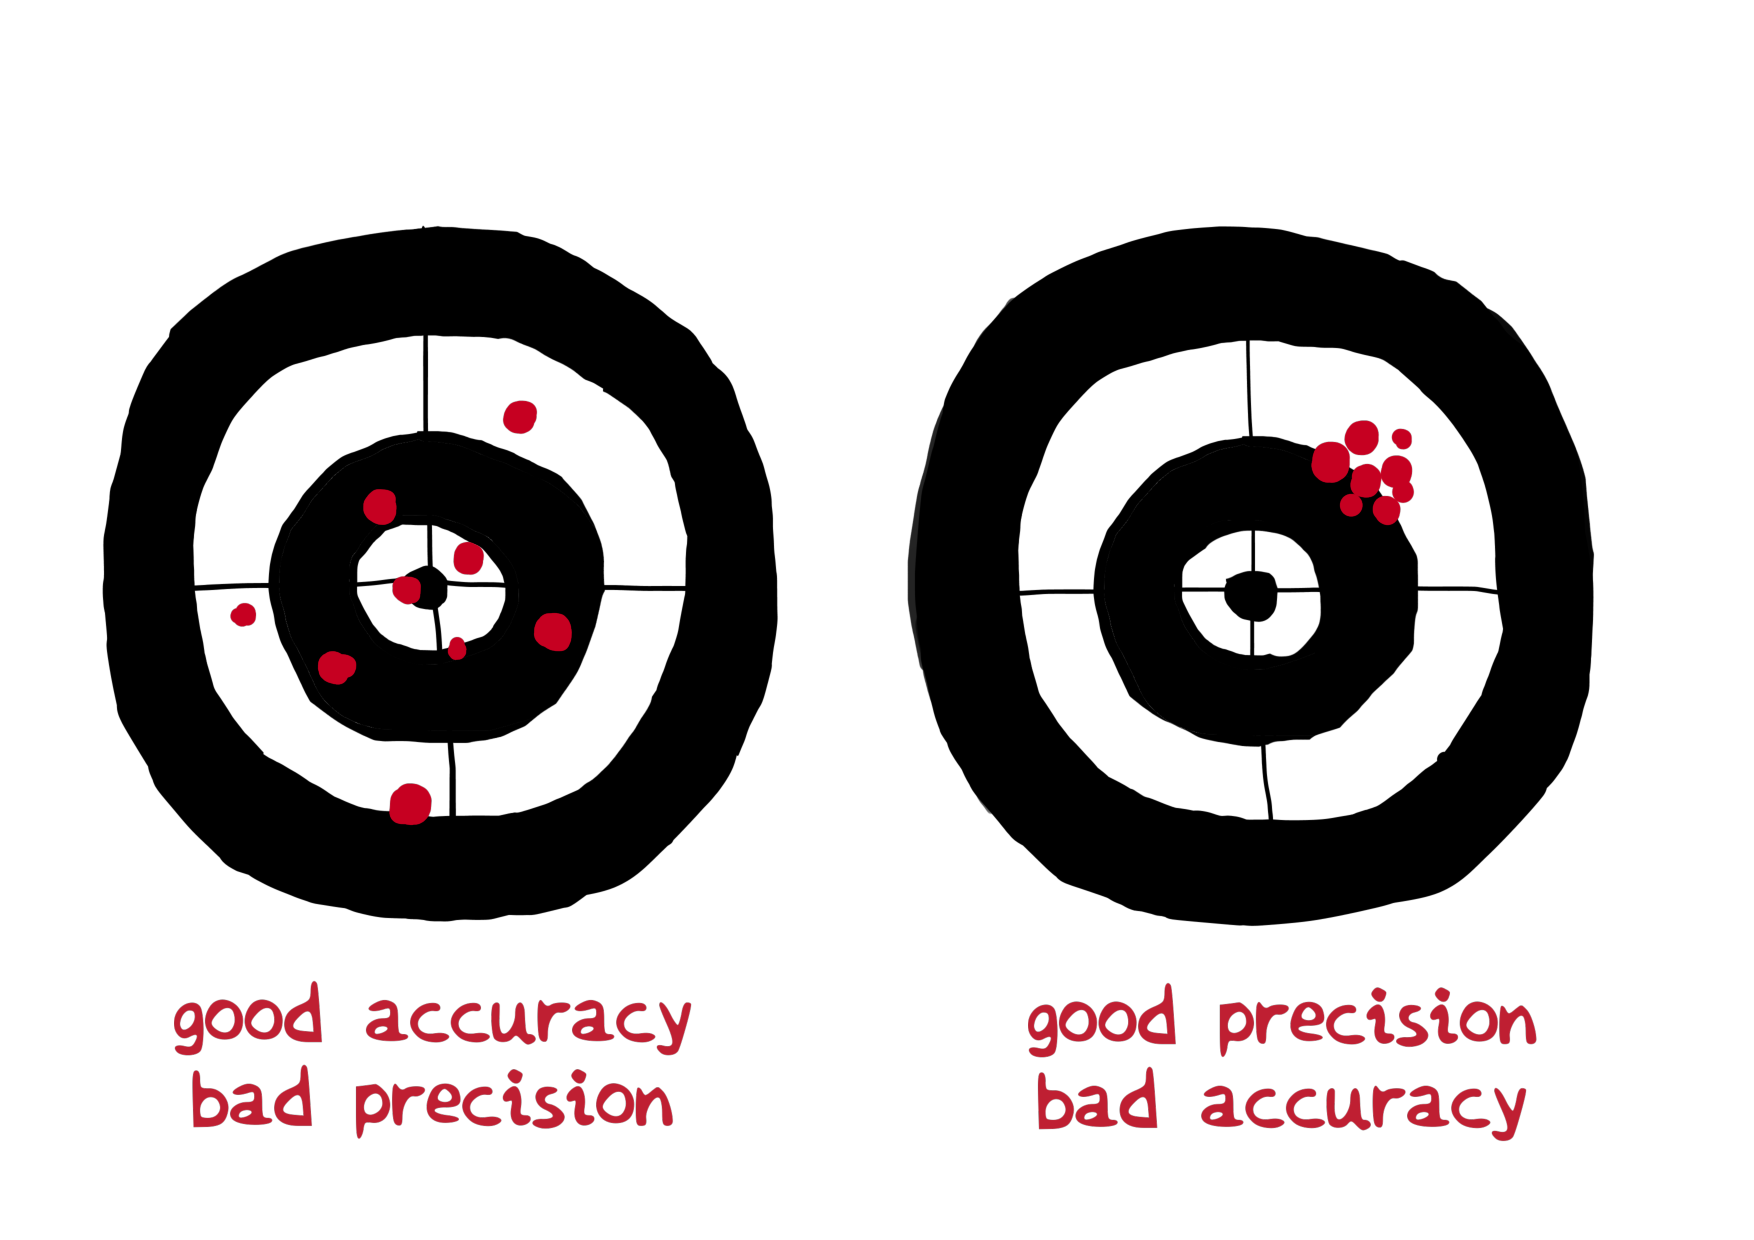
\includegraphics[width=0.7\linewidth]{accuracy.pdf}
	\vskip -0.5cm
	\caption{Illustration of the difference between precise and accurate data.}
	\label{fig:accuracy}
\end{figure}

\subsection{Classification of errors by reason of their occurrence}
\definition{Error of equipment} is caused by fundamental imperfections of the set up. The reason can be the equipment itself (e.g a fast or slow stop-watch) or improper use of the equipment (e.g wrong calibration). This error is \textit{systematic}.

\example{} Bad graded ruler, slow or fast watch, bad calibration of the set up.
\newline
\newline
\definition{Roundoff error} appears because of the result you get from any device (both analog or digital) has a finite number of significant digits. This error can be classified as a \textit{random} error since if one performs a lot of measurements then it is equally likely that rounding off will increase and decrease the value. If there is no other source of random errors in the experiment then the device will however show the same result all the time and roundoff error becomes a \textit{systematic} one.

\example{part I} Let's assume you have quite strange scientific calculator with only 4 digits on the screen. If you now want to get value of $\pi$ it shows you 3.141 (or 3.142) while $pi$ has infinite numbers of digits.
\newline
\newline
\definition{Error of calculations} is similar to the roundoff error but now we are talking about rounding off during the calculations.

\example{part II} Now you want to divide your $\pi$ over 1 000. It should be 0.003141 but since you calculator shows only 4 digits you will see 0.003. You might think that it is not a big problem, but now try to divide $\pi$ over 10 000. Instead of 0.0003141 you will get just 0!

Of course real calculators have more digits on the screen. And moreover they work with significant digits (see section \ref{sign_digits}) only. But as we said $\pi$, for example, has infinite number of significant digits so if you want to have $\pi^2$ you will face error of calculations again.

Representing numbers with finite number of significant digits is a big problem in computer science as well.
\newline
\newline
\definition{Error of method} is caused by imperfections of the method we use in the experiment. In any physical problem, we have to use some model. It means that we have to neglect some phenomena in order to be able to solve the problem. These errors give \textit{systematic} contributions.

\example {} Not taking into account air resistance in experiments with falling bodies.
\newline
\newline
\definition{Subjective error} is an error caused by the human who perform the experiment.  In an experiment with a stop-watch, for example, all times will be overestimated because of the reaction time. Then we deal with \textit{systematic} errors. Subjective errors can give a contribution to \textit{random} errors as well. If one have to estimate half of a distance  with the bare eye, for example, then the result can be biased in both sites.

\example{} The reaction time (0.3 s) should be taken into account if you use manual stop-watch. 
\newline
\newline
\definition{Mistakes} (or illegitimate errors) are rough errors which can occur as a result of misreading the data, algebraic mistakes, damaged devices etc. These errors are usually apparent either as obviously incorrect data points or as results that are not reasonably close to the expected values. Mistakes can be corrected by carefully repeating the operations.

%----------------------------------------------------------------------------------------
%	Scientific Notation
%----------------------------------------------------------------------------------------
\section{Quoting the Result and Scientific Notation}
\definition{Uncertainty} is the final error, after considering contributions from all errors above. Usually it is denoted by $\sigma$. It is computed as
\begin{equation} \label{sigma_tot}
\boxed{\sigma_{tot} = \sqrt{\sigma_1^2+\sigma_2^2 + ...}}
\end{equation}
where $\sigma_1, \sigma_2, ...$ are different types of errors which we assume to occur independently.
\newline
\newline
\definition{Discrepancy} is the difference between two results. Either you compare two experimental results or the experimental result with the accepted value of the physical quantity.

We will now discuss how to write down physical quantities together with their uncertainties in a correct way (how to compute the errors we will discuss in the next chapters).

\subsection{Rounding off}
When some digits are dropped from a number, the last digit retained should be rounded off for the best accuracy. For example we want to round off 1.2345 to the third digit. Then the fraction after the third digit 0.45 will define the way how we should do this according the following rules:
\begin{enumerate}
\item If the fraction is greater than $\frac{1}{2}$ , increment the last digit.
\item If the fraction is less than $\frac{1}{2}$, do not increment.
\item If the fraction equals $\frac{1}{2}$, increment the last digit only if it is odd.
\end{enumerate}

The last rule reduces systematic error in rounding off numbers.

\subsection{Significant digits}\label{sign_digits}
There are 4 rules for significant figures (let's consider number 12.34):
\begin{enumerate}
\item The leftmost nonzero digit is the most significant digit~(1).
\item If there is no decimal point, the rightmost nonzero digit is the least significant digit (it is not our case)
\item If there is a decimal point, the rightmost digit is the least significant digit, even if it is a~0~(4).
\item All digits between the least and the most significant digit are counted as significant digits~(2, 3).
\end{enumerate}
 So we have 4 significant digits in number 12.34. Here are other numbers with 4 significant digits:
 \begin{equation*}
 1234;\;\;\;\;1 234 000; \;\;\;\;1.234;\;\;\;\; 0.001234;\;\; \;\;0.01200;\;\;\;\; 123.0;\;\;\;\; 1.000
  \end{equation*}
  
\textbf{Note, that numbers 123 and 123.0 are mathematically equal but they have different numbers of significant digits!}. 123.0 is more \textit{precise} than 123.

\subsection{Quote the result}
Let's assume that your have already got some result in the experiment and calculated the uncertainty. We will show how the result can be quoted together with the error in the following table

\begin{center}
  \begin{tabular}{| p{2.7cm}|  p{3.9cm} | p{9cm} | }
    \hline
    Result & Answer & Comments\\ \hline  \hline
    \vspace{0.4 cm}{$ L = 2.5492$ m $\sigma = 0.03$ m} &\vspace{0.5 cm}$L = (2.55 \pm 0.03)$ m & We have uncertainty in the third digit, i.e. in number ``4" in our result. So the rest of the digits don't make sense. We should truncate the answer to those digits where we have our uncertainty. \\ \hline
    \vspace{0.4 cm}$ L = 77.323$ m  $\sigma = 0.82$ m & \vspace{0.5 cm}$L = (77.3 \pm 0.8)$ m & Here we have corrections to two digits in the result but the first significant digit in the error is larger than the second one. Then we can round off the result. \\ \hline
      \vspace{0.4 cm}$ L = 77.323$ m\;\;  $\sigma = 0.28$ m& \vspace{0.5 cm}$L = (77.32 \pm 0.28)$ m & The opposite situation: the first significant digit in the error is  smaller then the second one. We can keep it then.\\ \hline
   \vspace{0.4 cm}$ T = 1322.7$ s\;\;  $\sigma = 72.33$ s & \vspace{0.5 cm}$T = (1320 \pm 70)$ s & Round off to the first significant digit in the uncertainty. We have to leave the zero, since $70\neq7$.\\ \hline

  \end{tabular}
\end{center}

The last example reveals an interesting problem. We have only one significant digit in the error but we have to keep one more digit (it is not significant even) only because $70\neq7$. This leads us to the necessity to use \textit{scientific notation} for writing down numbers.

\subsection{Scientific notation}
In scientific notation a number is written on form: $m$ times ten raised to the power of  $n$, that is
\begin{equation*}
m\times 10^n, 
\end{equation*}
where the coefficient $m$ is any real number (called the significand or mantissa) and the exponent $n$ is an integer (can be both positive and negative).

The table below might help to understand the idea.

\begin{center}
  \begin{tabular}{ | p{3cm} | p{4cm} |}
  \hline
    Value & Scientific notation\\ \hline  \hline
    \vspace{0.02cm} 1000 & \vspace{0.02 cm}$1.0\cdot10^3$ \\ \hline
    \vspace{0.02cm} 0.001 & \vspace{0.02cm} $1.0\cdot10^{-3}$ \\ \hline
    \vspace{0.02cm} 237.83 & \vspace{0.02cm} $2.3783\cdot10^{2}$ \\\hline
    \vspace{0.02cm} $24.06\cdot10^{8}$&\vspace{0.02cm}  $2.4606\cdot10^{9}$ \\ \hline
    \vspace{0.02cm} $0.003\cdot10^{8}$&\vspace{0.02cm}  $3.0\cdot10^{5}$ \\ \hline
    \vspace{0.02cm} $0.045\cdot10^{-12}$&\vspace{0.02cm}  $4.5\cdot10^{-14}$ \\ \hline
    
  \end{tabular}
\end{center}

%----------------------------------------------------------------------------------------
%	Calculation of Errors in Direct Experiment
%----------------------------------------------------------------------------------------
\section{Calculation of Errors in Direct Experiment }
A \definition{direct measurement} is a measurement where you obtain the desired quantity itself and do not do any kind of calculations.

\example{} measuring the length of a stick with ruler. If you instead would like to find half the length by dividing by 2 then it would be an indirect measurement. This case will be discussed in the next chapter.

You can find examples of calculation errors in chapter \ref{example}.

\subsection{Average}
In a lot of experiments you need to find only one value. In this case usually you do the same measurement under the same conditions several times in order to increase the precision of the result. Then the unknown quantity should be calculated as the average over all outcomes: 

\begin{equation}
\label{av}
\boxed{\langle x\rangle = \frac{1}{N}\sum_{i=1}^N x_i}
\end{equation}

The error of this quantity should be found as \definition{standard deviation of average}:
\begin{equation}
 \label{av_error}
\boxed{S_{\langle x\rangle} =\sqrt{ \frac{1}{N(N-1)}\sum_{i=1}^N (x_i-\langle x\rangle)^2} = \sqrt{\frac{1}{N}}S_x}
\end{equation}

where $S_x = \sqrt{ \frac{1}{N-1}\sum_{i=1}^N (x_i-\langle x\rangle)^2}$ is a \definition{standard deviation} of \textbf{one certain} measurement. It means that if you want to know the deviation of your third, for example, measurement from set of, say, 5 measurements then you use $S_x$ with parameters $i = 3,\;N=5$. The error of average, not of a single measurement, is given by equation \ref{av_error}.

Why it is so important not to mix up $S_x$ and $S_{\langle x\rangle}$? In mathematical statistics it is shown than with increasing $N$, $S_x$ tends to a constant value. Hence, $S_{\langle x\rangle}$ tends to 0:
\begin{equation}
\lim_{N\rightarrow\infty}S_x=\rm{Const} \Rightarrow \lim_{N\rightarrow\infty}S_{\langle x\rangle}=0
\end{equation}
It means that indeed, with an increasing number of measurements you will decrease random errors and increase the precision of the experiment. It can be reflected only with the correct formula \ref{av_error}.

\subsection{Least Square Fit}
Suppose that you have a spring and want to find the spring constant, having a set of blocks with different masses and a ruler. According to the Hooke's law:

\begin{equation} \label{Hooke}
\vert\vec{F}\vert = k\vert\Delta x\vert
\end{equation}
In principle, you could make a set of measurements when you use only one block and measure the difference in the length of the spring. Then you would find the coefficient $k$ as a result of indirect measurements (see section \ref{indirect_meas}).

There is however a more efficient way to find $k$. Instead of using only one block you could use different ones with different masses. Hence you will have a table with weights $F_i$ and the corresponding $\Delta x_i$. Theoretically all the data points should belong to the line (\ref{Hooke}), and the slope would be the desired spring constant $k$. But as we already know, the real experiment always has errors. In this case it means that the data points will \textit{approximate} the line (\ref{Hooke}) but not strictly belong to it.

\definition{Least square fit} is the most common way of fitting the data with any (not only linear) functions.
Despite that the idea behind the least square method is simple, a proper description would be lengthy. For now just note, that least square fit is a part of \textit{linear regression method}.
%maybe give a reference such that the interested student could read more

Most likely you will do the fitting of your data by using some software\footnote{Scientific calculators are able to do linear fitting as well.} such as GNUplot, Matlab, Mathematica etc. All these programs are able to do this for you. You can learn more by reading the description of particular function you are going to use.  Unfortunately, a lot of programs don't present errors of fitting by default, so you have to call some extra functions.

Errors of fitting are really important, because in principle you can fit whatever data with whatever function, only errors \footnote{$\chi$-square test is also important for estimation of fitting quality. But this topic lies beyond the scope of this booklet.} will show you how good your fitting function is. The plot of a function together with the data is also useful, but it can only give subjective information, while quantitative estimation is objective information. Take a look at Figure \ref{fig:fitting}. There you can see how different data are fitted with the same line.

Whatever software and function you decide to use \textbf{you must present the error of fitting together with the result}.
\begin{figure} \label{fig:fitting}
	\centering
	\vskip -1cm
	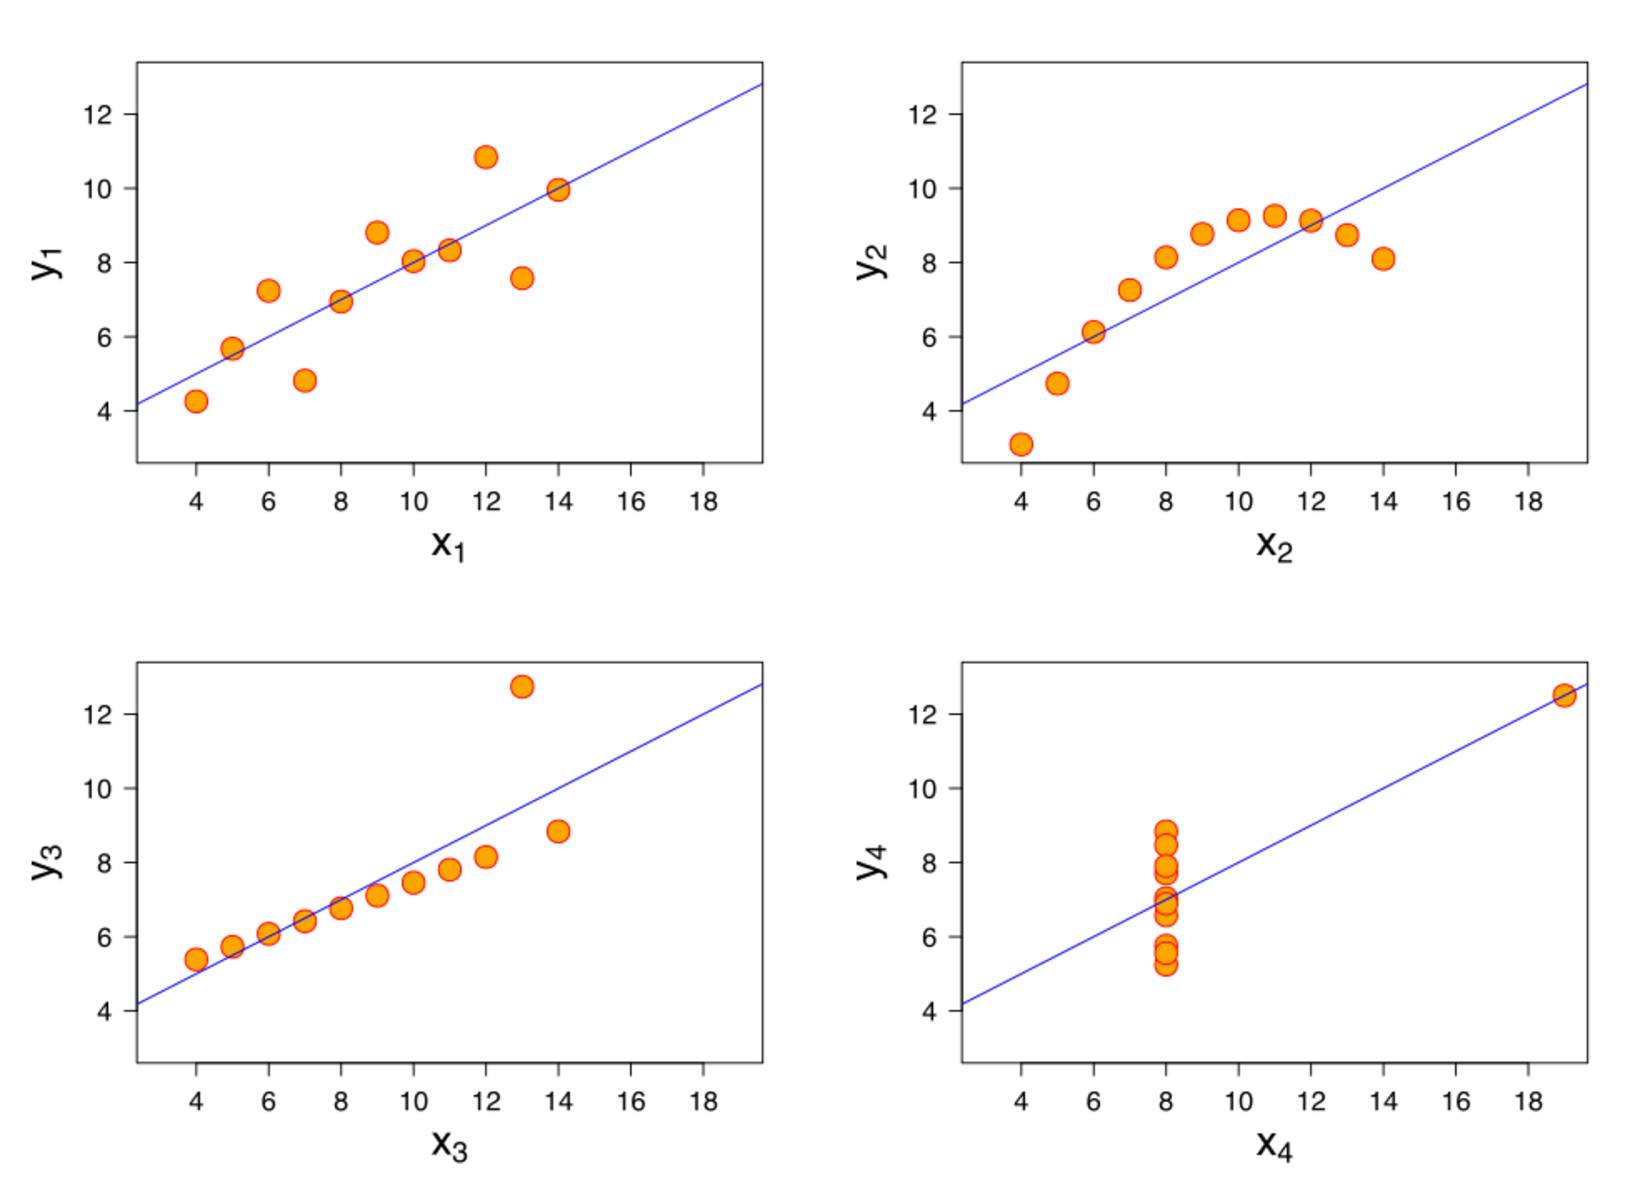
\includegraphics[width=.9\linewidth]{Anscombe's_quartet_3.pdf}
	\vskip -0.5cm
	\caption[]{Illustration how the same linear regression line fits different data sets \protect\footnotemark.}
\end{figure}
\footnotetext{Reference to the picture: Anscombe, Francis J. (1973) Graphs in statistical analysis. American Statistician, 27, 17–21}

Let us come back to our example with spring constant. In that case you want to approximate the data with a line:
\begin{equation}
y = ax + b
\end{equation}
where $y = F$ and $x = \Delta x$. Hopefully the coefficient $b$ will be very small, then we can say that the Hooke's law works well in our case and the answer for stiffness is:
\begin{equation}
k = a\pm \sigma_a\;[\rm{units}]
\end{equation}

The coefficient $b$ and its error are not the part of the result, however do not forget to check them as well. If $b$ is not close to zero or the error is very big then it might be a signal that you made a mistake somewhere and have to fix it.

\subsection{Peaks}
In some experiments you want to measure quantities which are given to you as a peak in the measured result (e.g. wave length). Ideally you want to obtain a delta-function, where the height show the intensity of the signal and the position is the required quantity. Real equipment cannot give you this ideal precision. Instead of the desired delta-function you will have a Gaussian distribution \footnote{Strictly speaking, it can be some other distribution as well, but in the overwhelming majority of cases it would be a Gaussian distribution.}:
\begin{equation}
P_G(\mu, \sigma) = \frac{1}{\sigma \sqrt{2\pi}}\exp\left\lbrace\frac{1}{2}\left(\frac{x-\mu}{\sigma}\right)^2\right\rbrace
\end{equation}

$\mu$ is \textit{mean-} or \textit{expectation value} and this is the value of our desired quantity. 

$\sigma$ is a \textit{standard deviation}, which give us the uncertainty of the measurement.
You need then to fit your data with a Gaussian distribution and find $\mu$ and $\sigma$ as the parameters of the fit. However, this way of doing it would be quite complicated, you would need some additional software which allows you to do this kind of fitting. In many cases (when you are not so interested in the precision of error) one can use this trick to find the standard deviation.

There is a value $\Gamma$ which denotes the \textit{full-width at the half maximum} or \textit{half-width}.
\begin{equation}
P_G(\mu\pm\frac{1}{2}\Gamma,\sigma) = \frac{1}{2}P_G(\mu, \sigma)
\end{equation}
It can be shown that $\Gamma$ has the property,
\begin{equation}
\Gamma = 2.354\,\sigma.
\end{equation}
It means that in the first approximation \textbf{you can count the error as a half-width at the half maximum of the peak}.
\begin{figure}[H]
	\centering
	\vskip -0.5cm
	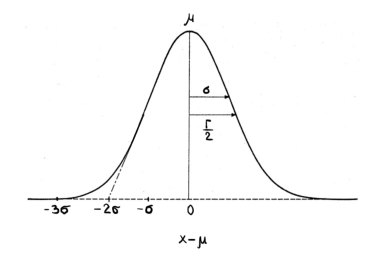
\includegraphics[width=.7\linewidth]{gauss_croped.pdf}
	\vskip -0.5cm
	\caption{Gaussian probability distribution.}
\end{figure}

%----------------------------------------------------------------------------------------
%	Calculation of Errors in Indirect Experiment
%----------------------------------------------------------------------------------------
\section{Calculation of Errors in Indirect Experiment }\label{indirect_meas}
If you do any kind of mathematical operations with a measured quantity then we say that the result was measured indirectly. Or that you did an \definition{indirect measurement}. 

\example{} you measured two sequent time intervals. The total time which is just the sum of those intervals will be an indirect measurement.

In general, an indirect quantity $u$ depends on direct quantities $x, y, z$ (could be any number of quantities) as some function:
\begin{equation}
u = f(x,y,z)
\end{equation}
The random error can then be calculated as a function of the direct quantities and their errors like this:
\begin{equation}\label{indirect_err}
\boxed{S_u = \sqrt{\left(\frac{\partial f}{\partial x}\right)^2\cdot S_{\langle x\rangle}^2+\left(\frac{\partial f}{\partial y}\right)^2\cdot S_{\langle y\rangle}^2+\left(\frac{\partial f}{\partial z}\right)^2\cdot S_{\langle z\rangle}^2}}
\end{equation}
where $\frac{\partial f}{\partial i}$ is a partial derivative. For systematic errors the equation is the same but instead of random errors for direct measurements $S_{\langle i\rangle}$ one should take systematic ones $\sigma_{\langle i\rangle}$.

In the next chapter you can learn how to deal with this case by one simple example.

\section{Example and Important Remark} \label{example}
Let's consider one simple example which covers a lot of what we have discussed above.

Kristofer wants to find the frequency of a swinging pendulum. He measures the time $t$ for n=50 periods of the pendulum and then use the formula:
\begin{equation}\label{nu}
\nu = \frac{n}{t}
\end{equation}

He repeats the measurement $N=5$ times and puts his results into the table:
\begin{center}
  \begin{tabular}{ | p{0.5cm} | p{1cm}|}
    \hline
  	No. & t (s) \\ \hline
    \hline
    \vspace{0.01cm} 1 & \vspace{0.01cm}105.7 \\ \hline
    \vspace{0.01cm} 2 & \vspace{0.01cm}106,5 \\ \hline
    \vspace{0.01cm} 3 & \vspace{0.01cm}105.9 \\\hline
    \vspace{0.01cm} 4 & \vspace{0.01cm}109.2 \\ \hline
    \vspace{0.01cm} 5 & \vspace{0.01cm}110.0 \\ \hline
  \end{tabular}
\end{center}

The average according to eq. \ref{av} is:
\begin{equation}
\langle t\rangle = \frac{1}{N}\sum_{i=1}^N t_i = \frac{537.3}{5}=107.46\;s
\end{equation}
In order to calculate the standard deviation of the average (eq. \ref{av_error}), it is convenient to add an extra column to the table for $(t_i-\langle t\rangle)^2$ :

\begin{center}
  \begin{tabular}{ | p{0.5cm} | p{1cm} |p{2.5cm}|}
    \hline
  	No. & t (s) & $(t_i-\langle t\rangle)^2\;\left(s^2\right)$ \\ \hline
    \hline
    \vspace{0.01cm} 1 & \vspace{0.01cm}105.7 & \vspace{0.01cm}3.0976\\ \hline
    \vspace{0.01cm} 2 & \vspace{0.01cm}106.5 & \vspace{0.01cm}0.9216\\ \hline
    \vspace{0.01cm} 3 & \vspace{0.01cm}105.9 & \vspace{0.01cm}2.4336\\\hline
    \vspace{0.01cm} 4 & \vspace{0.01cm}109.2 & \vspace{0.01cm}3.0276\\ \hline
    \vspace{0.01cm} 5 & \vspace{0.01cm}110.0 & \vspace{0.01cm}6.4516\\ \hline
  \end{tabular}
\end{center}
The error is found as:
\begin{equation}
S_{\langle t\rangle} =\sqrt{ \frac{1}{N(N-1)}\sum_{i=1}^N (t_i-\langle t\rangle)^2} = 0.8925245\;s
\end{equation}
Note that Kristofer left more digits than needed, because he will use this number for further calculations. He will do a proper roundoff at the end.

The expectation value for the frequency is:
\begin{equation}
\langle\nu\rangle= \frac{n}{\langle t\rangle} = 0.465289 \;\frac{1}{s}
\end{equation}

Random errors for indirect measurement (eq. \ref{indirect_err}) can be calculated as:
\begin{equation}
S_{\langle \nu \rangle} = \sqrt{\left(\frac{\partial \nu}{\partial t}\right)^2\cdot S_{\langle t\rangle}^2} = \sqrt{\left(\frac{-n}{\langle t\rangle^2}\right)^2\cdot S_{\langle t\rangle}^2} = 0.0038644
\end{equation}

Now Kristofer wants to take into account systematic errors. He assumes that equipment error can be neglected because it is much smaller than the reaction time: $\sigma_{react} = 0.3\;s$

Using the same formula, but for systematic errors, he gets:
\begin{equation}
\sigma_{\langle \nu \rangle}  = \sqrt{\left(\frac{-n}{\langle t\rangle^2}\right)^2\cdot \sigma_{\langle t\rangle}^2} = 0.00237
\end{equation}

Finally he finds the uncertainty using eq. \ref{sigma_tot}:
\begin{equation}
\sigma_{\langle \nu \rangle}^{tot}= \sqrt{S_{\langle \nu \rangle}^2+\sigma_{\langle \nu \rangle}^2} = 0.0045
\end{equation}

Then Kristofer presents the result of his experiment:
\begin{equation}
\nu = 0.465 \pm 0.005\;s^{-1}
\end{equation}	

\subsection{Very Important Remark}
The uncertainty in the example is quite small, only in the third digit. One can doubt if the real value of the frequency indeed lies in the interval $[0.460\,,\,0.470]$? The answer is more likely \textit{no} and \textit{probably it should not}! From the first sight it seems we contradict our own definition of uncertainty from the beginning of the booklet but let us look closer.

As you remember, when we discussed random errors, we always referred to statistics. Everything here should be understood by means of probabilities.

First of all, we mentioned the law of large numbers when we talked about equation \ref{av_error}, for example. It means that the theory was developed for a number of measurements $N \rightarrow\infty$. In our example Kristofer has only $N=5$ independent measurements, which is very far from infinity.

The second, even if $N$ is large enough the probability that the true value lies in the interval $[\langle x\rangle - \sigma\,,\,\langle x\rangle + \sigma]$ is only about 70\%! Even for this idealistic case, where  $N \rightarrow\infty$ we can get 100\% probability  for the true value only in the interval $[\langle x\rangle - \infty\,,\,\langle x\rangle + \infty]$. However, it is possible to increase the probability up to 99\%.

This subject lies beyond the scope of the booklet, but you can search for \textit{confidence intervals}.

In practice in order to take into account both a limited number of measurements and a probability distribution, one can multiply the final uncertainty by some known coefficient. Search for \textit{Student's coefficient} for example.

For the laboratory works you do not need these more advanced methods for error propagation but be sure that you understand why the true value can lie outside the interval $[\langle x\rangle - \sigma\,,\,\langle x\rangle + \sigma]$. And be ready to explain it.

\section*{Acknowledgements}
I would like to thank Johann Schmidt and Tomas L{\"o}thman for productive discussions. As well as Lisa Freyhult and Peter Oppeneer for their corrections.
%----------------------------------------------------------------------------------------
%	BIBLIOGRAPHY
%----------------------------------------------------------------------------------------
\begin{thebibliography}{9}
 \bibitem{1}
	\begin{otherlanguage}{russian}
  	Митин И.В, Русаков В.С. \textit{Анализ и обработка экспериментальных данных}. -			 М.:НЭВЦ ФИПТ. 1998. - 48с.
  	\end{otherlanguage}
  	(Russian). Available online in Russian: http://ffmgu.ru/images/4/4c/Mitin\_rusakov.pdf
  \bibitem{2}
  Philip R. Bevington, D. Keith Robinson. (2003). \textit{Data reduction and error analysis for the physical sciences. Third edition.} New York, NY: McGraw-Hill.
  \bibitem{3}
 	Wikipedia - the free encyclopaedia. http://www.wikipedia.org.
\end{thebibliography}
 
\end{document}